\chapter{Level 3: Network attacks}
We conducted two network attacks at this level: a TCP SYN Flood attack with IP spoofing and an ICMP Flood attack. The objective was to observe the impact of these attacks on the network and analyse the network traffic using Wireshark.

\section{TCP SYN Flood Attack with IP Spoofing}
We initiated a TCP SYN Flood attack with IP spoofing from the attacker machine, targeting one of the victim machines. Figure~\ref{fig:TCPSYNFloodAttackerPOV} illustrates the attacker's perspective during the attack, utilising the \texttt{hping3} tool to generate a flood of TCP SYN packets with spoofed source IP addresses.

\begin{figure}[H]
\centering
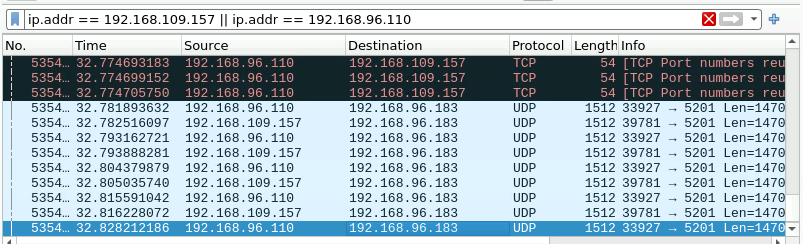
\includegraphics[width=0.8\textwidth]{img/level3/level3-attacker-TCPSYNFlood-pov.png}
\caption{TCP SYN Flood with IP Spoofing (Attacker)}\label{fig:TCPSYNFloodAttackerPOV}
\end{figure}

On victim 2's side, as depicted in Figure~\ref{fig:TCPSYNFloodVictimPOV}, we observed a high volume of incoming TCP SYN packets, indicating the impact of the flood attack. The victim machine attempted to respond with SYN-ACK packets. However, since the source IP addresses were spoofed to be those of Victim 1, the responses were sent to Victim one instead of the actual attacker, allowing us to perform a denial-of-service attack on both victim machines with a single attack, demonstrating a successful amplification attack.

\begin{figure}[H]
\centering
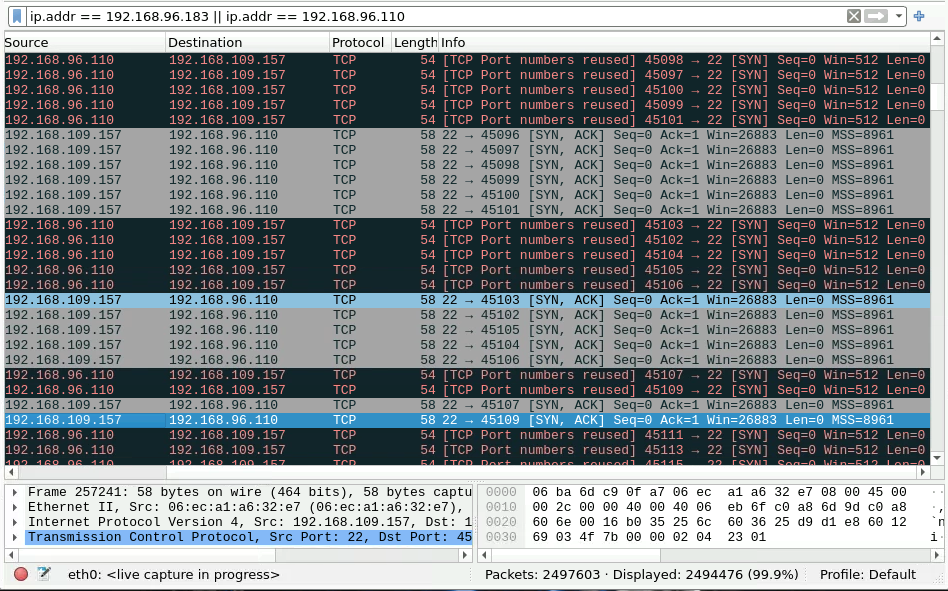
\includegraphics[width=0.8\textwidth]{img/level3/level3-victim1-TCPSYNFlood-pov.png}
\caption{TCP SYN Flood with IP Spoofing (Victim)}\label{fig:TCPSYNFloodVictimPOV}
\end{figure}

\section{ICMP Flood Attack}
We also executed an ICMP Flood attack from the attacker machine, simultaneously targeting both victim machines. Figure~\ref{fig:ICMPFloodAttackerPOV} showcases the attacker's perspective, employing the \texttt{hping3} tool to generate a high volume of ICMP echo request packets.

\begin{figure}[H]
\centering
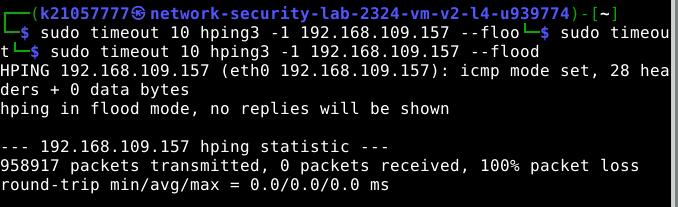
\includegraphics[width=0.8\textwidth]{img/level3/level3-attacker-ICMPFlood-pov.png}
\caption{ICMP Flood (Attacker)}\label{fig:ICMPFloodAttackerPOV}
\end{figure}

The victim machines were inundated with incoming ICMP echo requests, which consumed their resources and bandwidth as they attempted to process and respond to the flood of packets. This attack effectively overwhelmed the victim machines, impacting their ability to handle legitimate network traffic.

\section{Packet Analysis}
To assess the impact of the attacks on the network traffic, we captured packets using Wireshark during the attack scenarios. Figure~\ref{fig:PacketAnalysis} presents a sample of the captured packets.

\begin{figure}[H]
\centering
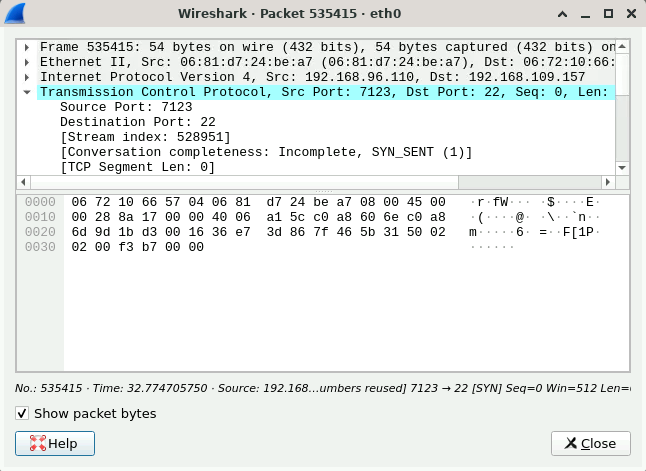
\includegraphics[width=0.8\textwidth]{img/level3/level3-packet-analysis.png}
\caption{Packet Analysis}\label{fig:PacketAnalysis}
\end{figure}

Upon closer examination of the TCP SYN packets, we discovered that the source IP addresses were spoofed, making it challenging for the victim machines to establish a complete TCP connection. Conversely, the ICMP echo request packets overwhelmed the victim machines with a barrage of requests, depleting their resources.

\section{Flow Analysis}
To gain deeper insights into the attack traffic patterns, we conducted flow analysis using Wireshark's Conversations feature. Figure~\ref{fig:FlowAnalysis1} presents the flow analysis for the TCP SYN Flood attack, highlighting the substantial number of TCP flows initiated by the attacker towards the victim machine.

\begin{figure}[H]
\centering
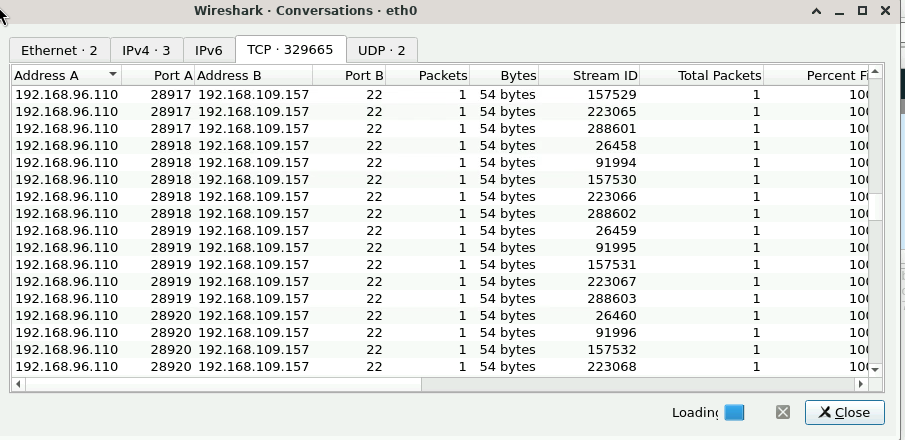
\includegraphics[width=0.8\textwidth]{img/level3/level3-flow-analysis1.png}
\caption{Flow Analysis 1}\label{fig:FlowAnalysis1}
\end{figure}

Similarly, Figure~\ref{fig:FlowAnalysis2} illustrates the flow analysis for the ICMP Flood attack, revealing the high volume of ICMP flows originating from the attacker and directed towards both victim machines.

\begin{figure}[H]
\centering
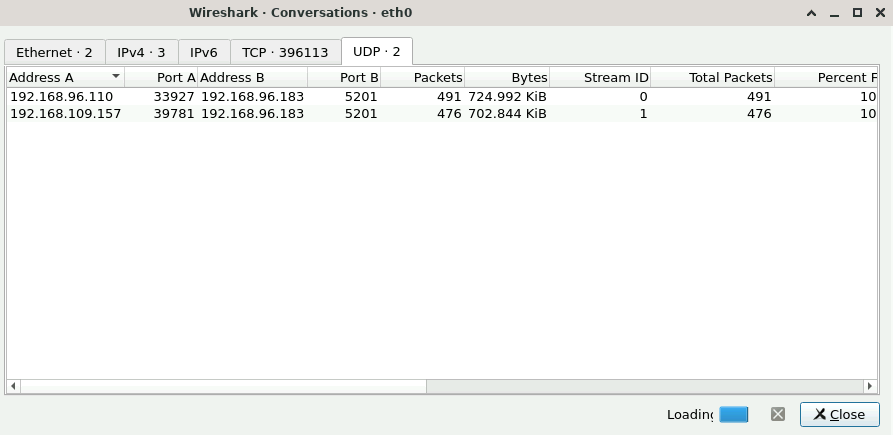
\includegraphics[width=0.8\textwidth]{img/level3/level3-flow-analysis2.png}
\caption{Flow Analysis 2}\label{fig:FlowAnalysis2}
\end{figure}

The flow analysis provides valuable insights into the intensity and distribution of the attack traffic, emphasising the significant impact on the targeted victim machines. By visualising the flow patterns, we can better understand the scale and effectiveness of the attacks.